\chapter{Application Layer}

\section{Introduzione al livello di applicazione}
È il livello \textbf{più alto} nello stack dei protocolli, ed è quello \textbf{più vicino all'utente}. È infatti il livello delle \textbf{applicazioni di rete}: la vastità delle funzionalità offerte dalle reti, è \textbf{alla base del successo di Internet}. \textbf{Trasferire e-mail o file}? \textbf{VoiP}? Comandare via \textbf{remoto} un altro computer? Questa è solo la punta dell'iceberg di ciò che le applicazioni di rete del livello applicativo ci permettono di fare. Come abbiamo già detto, il layer application sfrutta i layer inferiori: primo tra tutti, il livello di trasporto, di cui parleremo dopo. Ogni applicazione di rete si può basare su uno tra due paradigmi (o architetture). Il paradigma \textbf{Client-Server}, e il paradigma \textbf{Peer-to-Peer}.

\subsection{Paradigma Client-Server}
In questa architettura evidenziamo due attori principali: il \textbf{server}, un host sempre attivo che risponde alle richieste, e i \textbf{client}, host che mandano richieste al server. HTTP, IMAP, FTP sono alcuni tra i protocolli che sfruttano questo paradigma.

\begin{itemize}
    \item \textbf{Server.}\\
    (Se tutto va bene, solitamente) sempre attivo, ha un indirizzo IP\footnote{Un indirizzo IP permette di identificare univocamente un dispositivo su una rete.} statico che facilita l'accesso al server. Il server può essere un dispositivo o una struttura di più dispositivi (come in un data center). \textbf{Riceve richieste} e fornisce risposte.
    \item \textbf{Client.}\\
    \textbf{Manda richieste} al server. Può disconnettersi e (solitamente) ha un IP dinamico. In questa architettura, i client \textbf{non comunicano direttamente} tra loro. Ad esempio, i browser di due utenti (e quindi due client differenti) non comunicano mai direttamente tra loro. 
\end{itemize}


\subsection{Paradigma peer-to-peer}
In un'infrastruttura di rete potrebbe esserci la necessità di far comunicare \textbf{più client tra loro senza passare attraverso un server}: la comunicazione \textbf{peer-to-peer} permette ciò. I client sono \textbf{di pari livello}, ogni host (detto anche peer) può essere sia server che client.
È un'architettura scalabile, aggiungere un altro peer (nodo, partecipante alla comunicazione) è un processo immediato.\\
I peer non devono essere sempre accesi, e i loro indirizzi IP possono cambiare.\\
La comunicazione peer-to-peer ha come svantaggio la \textbf{complessità} in termini \textbf{di gestione} (lo scambio di pacchetti deve essere gestito in maniera consona per evitare errori) e il \textbf{forte impatto sulla banda} dei peer coinvolti. BitTorrent segue questo paradigma.

\subsection{Socket}
Un socket è un'interfaccia software che permette ad un processo di mandare dati verso la rete. Non sarebbe sbagliato immaginarli come delle porte, che possono essere aperte proprio tramite software: nello specifico, sono aperte tramite delle \textbf{primitive del sistema operativo}, il quale si occuperà della loro gestione indipendentemente dall'applicazione. I socket sono quindi a cavallo tra il livello applicativo e quello di trasporto, il quale non sarà oggetto di interesse (perlomeno, approfondito) da parte di un ipotetico sviluppatore di applicazioni di rete. Ogni connessione coinvolge sempre due socket, uno per lato.

\newpage

\subsection{Indirizzi IP e porte.}
Un host esegue $n$ processi. Un indirizzo IP (IPv4 o IPv6) identifica un host,\underline{ ma non il processo coinvolto}\\ \underline{nella connessione}: ne consegue che l'IP è identificativo (logico) per gli host, ma non per i processi degli host.
L'identificazione del processo di una macchina con IP noto, avviene tramite il numero di porta. 
\begin{verbatim}
    IP address: 128.119.245.12
    Port number: 80
\end{verbatim}

In questo esempio, la porta 80 è quella dedicata al protocollo HTTP, e sarà la porta di destinazione per le richieste ad un web server.

\subsubsection{In merito alle porte}
Un numero di porta è un intero a 16 bit, e si hanno quindi $2^{16}-1 = 65536$ porte possibili. I numeri di porta sono divisi in tre gruppi:
\begin{itemize}
    \item \textbf{Well Known Ports.}\\
    (0 - 1023) per servizi di sistema.
    \item \textbf{Registered Ports.}\\
    (1024 - 49151) sono assegnati dall'ICANN (Internet Corporation for Assigned Names and Numbers) per usi e servizi specifici.
    \item \textbf{Dynamic and/or Private Ports.}\\
    (49152-65535)
\end{itemize}

\subsubsection{Le porte dei protocolli studiati nel corso}
\begin{verbatim}
20 FTP - Data Port
21 FTP - Command Port
22 SSH 
23 Telnet
25 SMTP
53 DNS
80 HTTP
110 POP3
161 SNMP (Agent)
162 SNMP (Manager)
443 HTTPS
465 SMTP
994 POP3
\end{verbatim}

\subsection{Comunicazione inter-process e non}
Un processo è definito come un programma eseguito da un host.
\begin{itemize}
    \item I processi di uno stesso host possono comunicare tra loro tramite regole di \textbf{IPC}, definite dal sistema operativo.
    \item Due processi di due host differenti comunicano scambiando pacchetti, sfruttando i procolli del transport layer e quelli inferiori.
\end{itemize}

\newpage

\section{Definizione di un protocollo applicativo}
Un protocollo del livello applicativo è caratterizzato dalle seguenti caratteristiche
\begin{itemize}
    \item \textbf{Tipo di messaggi.}\\
    Come messaggi di richiesta e di risposta.
    \item \textbf{Sintassi dei messaggi.}\\
    I campi dei messaggi. Nei protocollo HTTP e SMTP, ad esempio, sono definiti dei campi ben precisi (alcuni di loro obbligatori).
    \item \textbf{Semantica dei messaggi.}\\
    Il significato delle informazioni all'interno dei campi e come interpretarli.
    \item \textbf{Regole} sul come e quando mandare e rispondere ai \\messaggi.
\end{itemize}
 Sono spiegati in \textbf{documenti tecnici RFC} (Request for Comments) pubblicati dall'IETF (Internet Engineering Task Force) e dall'Internet Society (ISOC). \textbf{Definiscono standard}, protocolli e best-practices per il funzionamento di Internet e delle reti di comunicazione.\\
 I protocolli possono essere \textbf{aperti} (come HTTP o SMTP) o \textbf{proprietari} (come quello di Skype).


\newpage

\section{Trasferimento dati - TCP e UDP}
Per offrire una spiegazione completa dell'application layer, diamo una breve introduzione a quelli che sono i protocolli del livello di trasporto maggiormente usati (quali TCP e UDP) per garantire il trasferimento delle informazioni. Ogni protocollo di trasporto ha le proprie specifiche, ed è scelto in maniera \textbf{opportuna} per l'applicazione che lo sfrutta:
\begin{itemize}
    \item \textbf{Integrità dei dati.}\\
    Posso permettermi di perdere dei dati? O necessito di un trasferimento totalmente lossless?
    \item \textbf{Throughput.}\\
    Quantità di dati trasferiti in un'unità di tempo. Larghezza di banda e distanza tra gli host influenzano questo valore.
    \item \textbf{Timing.}\\
    Posso avere della latenza o devo offrire un servizio quanto più responsivo e istantaneo possibile?
    \item \textbf{Sicurezza.}\\
    I dati possono essere trasmessi in chiaro? o richiedono una forma di crittografia?
\end{itemize}
Ad esempio, audio o video in \textbf{streaming} perdonano un \textbf{throughput variabile}, più basso e anche la \textbf{perdita di pacchetti}, a discapito della qualità. Una perdita di pacchetti è inaccettabile per il trasferimento di file e l'alta latenza non è ottimale per video conferenze o gaming.

TCP e UDP sono ad oggi protocolli del layer di trasporto più importanti. Introduciamoli in breve 

\subsection{TCP - Transmission Control Protocol}
Offre le seguenti specifiche:
\begin{itemize}
    \item \textbf{Trasporto affidabile}.\\ 
    (\textit{Reliable transport}) tra mittente e destinatario, tramite meccanismi di \textit{ACKnowledgment} dei pacchetti.
    \item \textbf{Controllo del flusso} (\textit{flow control}).\\
    Il mittente cercherà di \textbf{non sovraccaricare} il \textbf{ricevente}, per minimizzare la perdita di pacchetti.
    \item \textbf{Controllo della congestione} (\textit{congestion control}).\\
    La banda viene limitata quando la \textbf{rete è sovraccaricata}.
    \item \textbf{Connection oriented}.\\
    È richiesto un setup tra client e server per effettuare la connessione. Usa un three-way handshake per stabilire una connessione.
    \item \textbf{Non fornisce garanzie} sulla latenza, tantomeno sul minimo throughput e sulla sicurezza
\end{itemize}


\begin{figure}[htp]
    \centering
    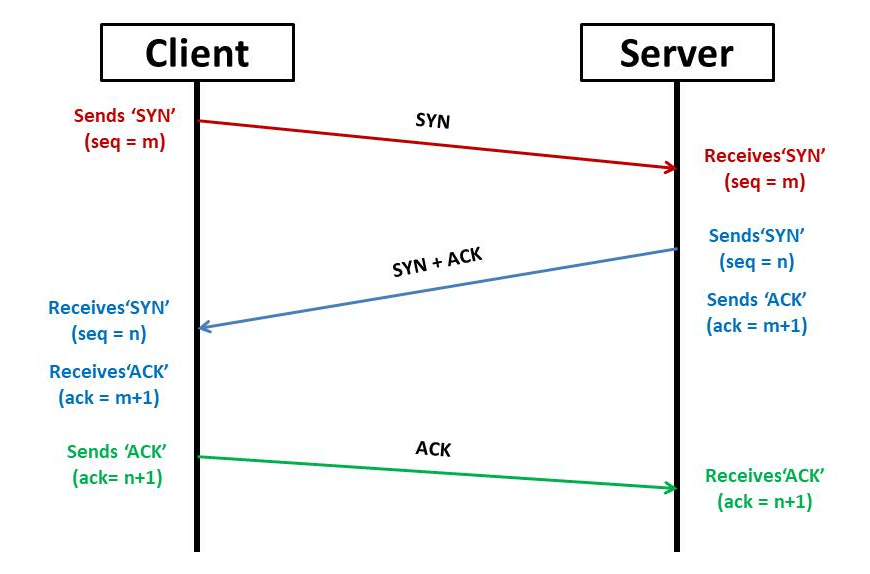
\includegraphics[width=0.75\linewidth]{./images/3wayhs.png}
    \caption{Three-way handshake}
\end{figure}

\newpage

\subsection{UDP - User Datagram Protocol}
È un protocollo minimal, scarno e \textit{unreliable}.

\begin{itemize}
    \item \textbf{Connectionless.}\\
    Non ha alcun tipo di handshake che stabilisca la connessione tra i due host.
    \item \textbf{Unreliable.}\\
    Nessuno scambio di ACK.
    \item \textbf{Nessun controllo del flusso.}\\
    UDP non gestisce il proprio throughput in funzione della congestione della rete, o del sovraccarico del receiver.
    \item \textbf{Nessuna garanzia sul throughput minimo.}    
\end{itemize}

UDP non è un protocollo sicuro: scopriremo però come il suo essere "ridotto all'osso", \textit{barebones}, sia il suo più grande punto di forza. È usato nei protocolli applicativi VoiP, streaming audio-video e gaming.


\newpage

\section{Telnet}
\textbf{Telnet} (da TErminaL NETwork) è un protocollo applicativo che permette di controllare il \textbf{terminale} di un altro host \textbf{da remoto}. 
\begin{figure}[htp]
    \centering
    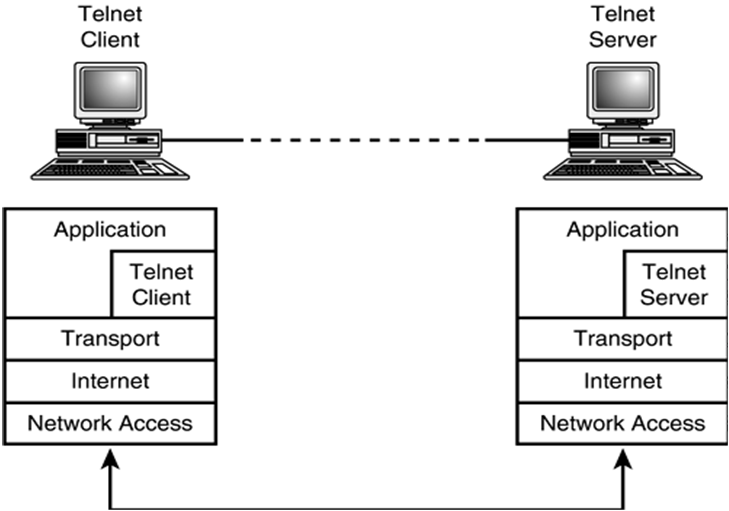
\includegraphics[width=0.5\linewidth]{./images/Requisiti di Telnet.png}
\end{figure}

È basato sul paradigma client-server (dove il pc remoto è il server), usa \textbf{TCP} la \textbf{porta 23} come porta destinataria (verso il server). 
Non è un protocollo sicuro: Telnet trasmette i dati (anche di autenticazione) in chiaro, l'autenticazione non è sempre obbligatoria, ed è vulnerabile a sniffing e man-in-the-middle. \textbf{SSH} (\textit{Secure Shell Protocol}) è simile al protocollo Telnet, ma sicuro, non trasmettendo i dati in chiaro. SSH usa la porta 22.

\subsection{Funzionamento di Telnet}
Basato sul protocollo di trasferimento TCP, Telnet sfrutta il three-way handshake per stabilire la connessione.
\begin{figure}[htp]
    \centering
    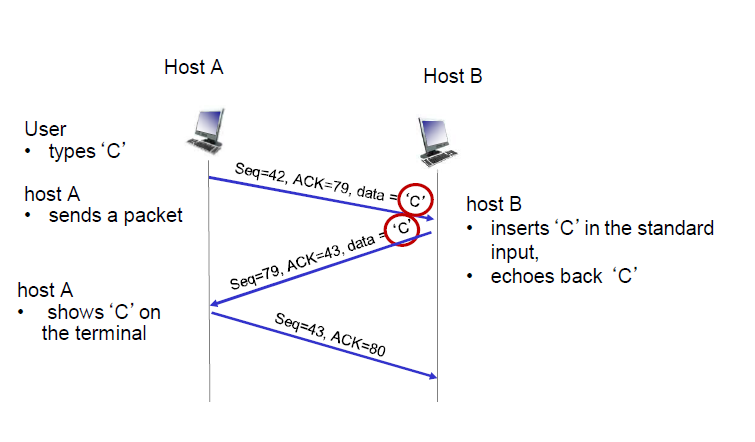
\includegraphics[width=0.75\linewidth]{./images/telnetscenario.png}
    \caption{Esempio di Telnet}
\end{figure}

Un fatto interessante è che Telnet può essere usato come strumento di debug per Server HTTP o Mail Server, inserendo come porta destinazione, una porta diversa dalla 23.


\subsection{Remote Desktop Protocol}
È un protocollo con presupposti simili a quelli di Telnet, ma che permette la trasmissione dell'intera interfaccia del dispositivo remoto.

\subsubsection{Telnet in breve}
Terminale remoto, TCP porta 23. Architettura client-server. Autenticazione trasmessa in chiaro, quindi non sicuro, sconsigliato e deprecato grazie ad SSH. SSH sfrutta la porta 22. 

\newpage

\section{FTP - File Transfer Protocol}
È un protocollo utilizzato per lo \textbf{scambio di file tra due host}. Basato sul paradigma \textbf{client-server}, sfrutta \textbf{TCP}. Offre inoltre un \textbf{meccanismo di autenticazione} (che avviene dopo lo stabilimento della connessione, ma precedentemente a qualsiasi scambio dati).

\subsection{Client-Server}
Col protocollo FTP, il client carica o scarica file verso o dal server. Il server ospita i file e gestisce le richieste.
La porta di controllo è la porta 21, su cui il server riceve le richieste. La porta del client usata per lo scambio dei dati è casuale, e trasmessa tramite il comando \verb|PORT|. La porta del server per lo scambio dati è la porta 20.

\begin{figure}[htp]
    \centering
    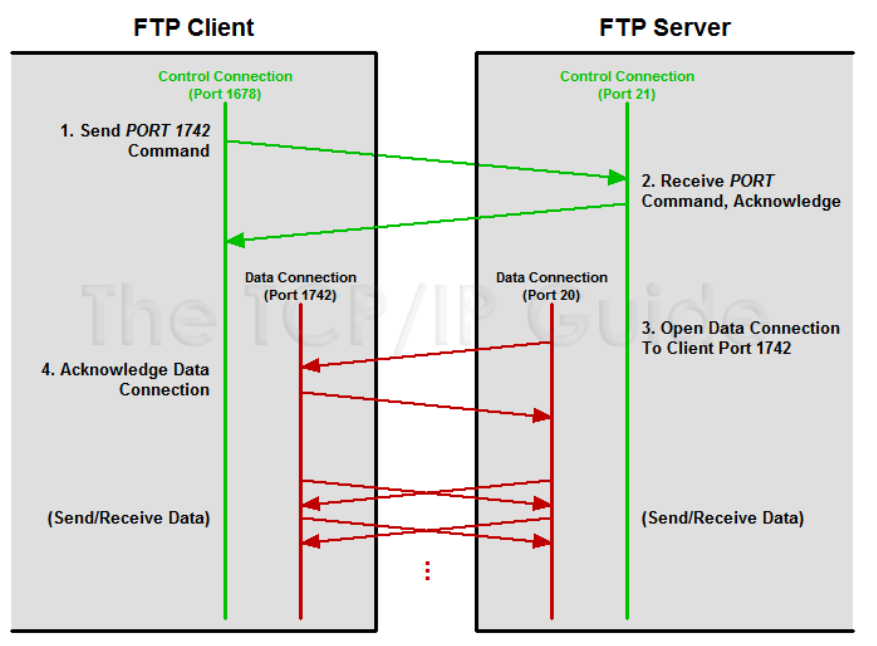
\includegraphics[width=0.75\linewidth]{./images/FTP.png}
    \caption{FTP}
\end{figure}

\subsection{Vulnerabilità del protocollo FTP}
\begin{itemize}
    \item Abilitare l'accesso all'intero file system tramite FTP è una mossa rischiosa: bisogna regolare quali porzioni rendere accessibili.
    \item Le credenziali di accesso e i dati (di default) sono trasmessi in chiaro, rendendo FTP vulnerabile ad attacchi man-in-the-middle e allo sniffing. Il protocollo \textbf{SFTP} risolve il problema implementando l'encryption di SSH. Usa la stessa porta di SSH, la porta 22.
\end{itemize}

\subsubsection{FTP in breve}
Upload e download di file su host remoto, TCP porta 21 (porta di controllo) e TCP porta 20 (porta dati) del server. Architettura client-server. Autenticazione e dati trasmessi in chiaro, quindi non sicuro, sconsigliato e deprecato grazie ad SFTP. SFTP sfrutta la porta di SSH, la porta 22. 

\newpage

\section{HTTP - HyperText Transfer Protocol}
\textbf{HTTP} permette ad un host di richiedere delle risorse, chiamate oggetti, ad un Web Server. Questi oggetti possono essere pagine HTML, file multimediali di vario tipo (e, col modello DHTML, affiancate alle pagine HTML, abbiamo anche fogli di stile CSS e file Javascript). Per accedere a queste risorse usiamo un URL (\textit{Uniform Resource Locator}). È quindi il protocollo alla base delle pagine Web, e segue (banalmente) l'architettura Client-Server.
La porta dedicata al protocollo, lato server, è la porta 80, ed è la porta da cui il server riceverà le richieste. Ricordiamo che la porta sorgente del client è stabilita (casualmente) dall'OS.

\begin{figure}[htp]
    \centering
    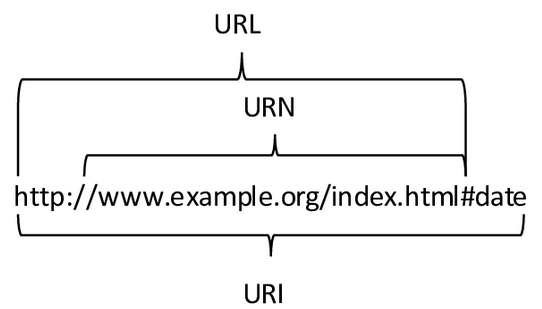
\includegraphics[width=0.6\linewidth]{./images/URL.png}
\end{figure}

\subsection{In cosa consiste la connessione HTTP}
HTTP utilizza TCP e il suo Three-Way Handshake.
\begin{enumerate}
    \item Il client \textbf{richiede la connessione TCP sulla porta 80} del server.
    \item Il \textbf{server accetta} la connessione TCP da parte del client.
    \item \textbf{Messaggi HTTP vengono scambiati} tra il browser (del client) e il web server (del server).
    \item \textbf{Si chiude la connessione} TCP.
\end{enumerate}

Questi passi avvengono in un tempo chiamato \textit{Round Trip Time (RTT)}.

\subsection{Versioni di HTTP}
Il vasto utilizzo di HTTP, ha portato alla creazione di molteplici versioni nel corso degli anni.
\begin{itemize}
    \item \textbf{HTTP/1.0}\\
    Ogni trasferimento di oggetto implica un'apertura e chiusura di una connessione TCP. \textbf{Per ogni oggetto, una connessione TCP dedicata}. Overhead per ogni oggetto.
    \item \textbf{HTTP/1.1}\\
    Usa una \textbf{connessione TCP persistente}. La connessione viene \textbf{aperta all'inizio del trasferimento} di tutti gli oggetti, e \textbf{chiusa alla fine}. Meno overhead, ma ogni download avviene in maniera sequenziale.
    \item \textbf{HTTP/2}\\
    Comprime gli header e effettua i download in parallelo. Riduce ulteriormente le tempistiche.
    \item \textbf{HTTP/3}\\
    Il più recente, introduce numerose innovazioni, tra cui l'uso del protocollo di trasferimento QUIC (creato su UDP!).
\end{itemize}

\subsubsection{HOL Blocking}
L'\textbf{Head-of-Line blocking} è un fenomeno che avviene quando più richieste di risorse HTTP sono in coda. In HTTP/1.1, se $O_1$, una richiesta di un oggetto molto grande, viene inserita prima della richiesta di 3 oggetti molto piccoli $O_2,O_3,O_4$, la priorità verrà data all'oggetto $O_1$, in quanto quest'ultimo è situato in testa.
In HTTP/2, un insieme di algoritmi di \textbf{valutazione della priorità} e \textbf{slicing} degli oggetti in porzioni più piccole, risolve l'HOL blocking minimizzando i tempi di attesa per ogni oggetto, migliorando la \textit{User Experience}.

\newpage

\subsection{Struttura di una richiesta HTTP}

\begin{itemize}
    
    \item \textbf{Request Line.}
    \begin{itemize}
    \item \textbf{Metodo.}\\
    Indica il tipo di richiesta effettuata dal client.
    \item \textbf{URL.}\\
    Esplicita la risorsa desiderata.
    \item \textbf{Versione.}
    Esplicita la versione del protocollo HTTP.
    \end{itemize}

    
    \item \textbf{Header lines.}\\
    Più righe contenenti coppie \verb|Nome campo: Valore|, una per riga.
    \item \textbf{Body.}\\
    Che permette di specificare ulteriori parametri.
\end{itemize}

\begin{figure}[htp]
    \centering
    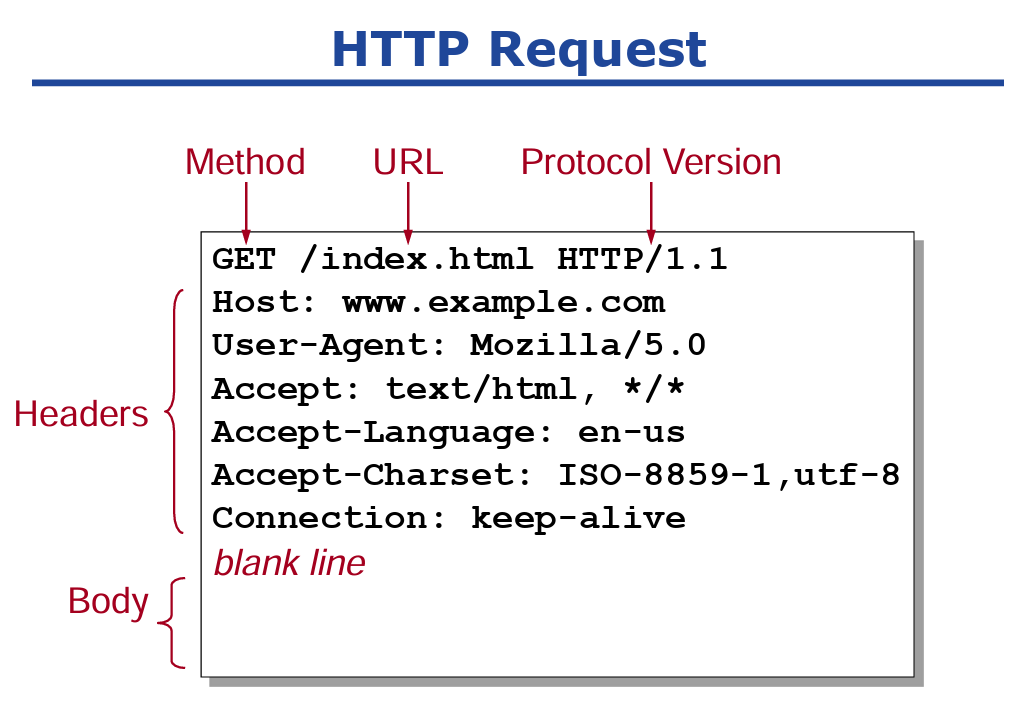
\includegraphics[width=0.75\linewidth]{./images/richiestahttp.png}
    \caption{Esempio di richiesta HTTP}
\end{figure}

\subsubsection{Alcuni metodi richieste HTTP}

\begin{itemize}
    \item \verb|GET|.\\
    Richiede dei dati dal server.
    \item \verb|POST|.\\
    Usato per mandare dei dati d'input da un client.
    \item \verb|HEAD|.\\
    Richiede esclusivamente l'header che sarebbe mandato da una richiesta HTTP \verb|GET| ad un determinato URL.
    \item \verb|PUT|.\\
    Usato per effettuare l'upload dei dati. Effettua un rimpiazzamento totale di un file che esiste a un determinato URL.
\end{itemize}

\newpage

\subsection{Struttura di una risposta HTTP}

\begin{itemize}
    
    \item \textbf{Status Line.}
    \begin{itemize}
    \item \textbf{Versione.}\\
    Ribadisce la versione del protocollo HTTP in uso.
    \item \textbf{Codice di stato.}\\
    Fornisce dettagli sulla corretta (o meno) elaborazione di una richiesta HTTP.
    \item \textbf{Messaggio di stato.}
    Esprime in linguaggio naturale il significato dello Status Code.
    \end{itemize}

    \item \textbf{Header lines.}\\
    Più righe contenenti coppie \verb|Nome campo: Valore|, una per riga.
    \item \textbf{Body.}\\
    Contiene i dati richiesti dal client nella rispettiva HTTP Request.
\end{itemize}

\begin{figure}[htp]
    \centering
    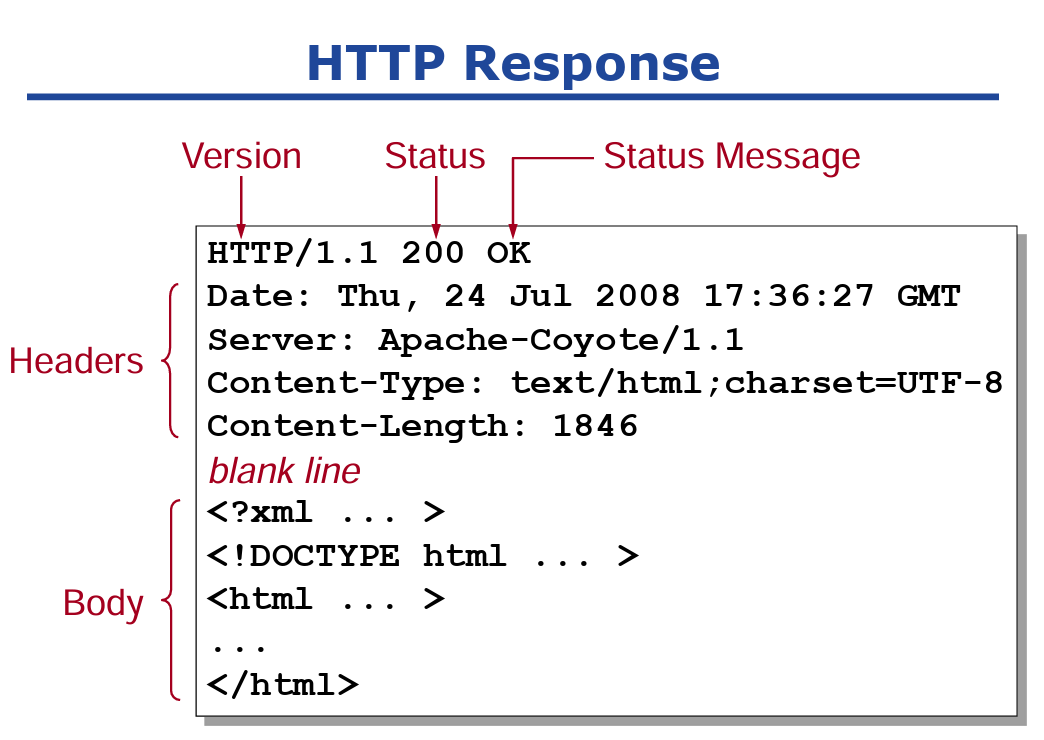
\includegraphics[width=0.75\linewidth]{./images/rispostahttp.png}
    \caption{Esempio di risposta HTTP}
\end{figure}


\subsubsection{Alcuni codici di risposta HTTP}
\begin{verbatim}
Information codes.
   100 Continue
   Success codes.
   200 OK
   203 Non-Authorative Information
   204 No Content
   
Redirection Codes.
   305 Use Proxy
   
Client Error Codes.
   400 Bad Request
   403 Forbidden
   404 Not Found
   405 Method Not Allowed
   
Server Error Codes.
   500 Internal Server Error
   505 HTTP Version Not Supported
\end{verbatim}

\newpage

\subsection{Parentesi Stateless, Stateful e Cookies}
Il protocollo HTTP è di default, un protocollo di tipo \textbf{stateless}. Tuttavia, con l'introduzione dei \textbf{cookies}, HTTP può memorizzare degli stati, diventando \textbf{stateful}\footnote{Un protocollo stateless può comunque avere un log delle azioni relative alle sessioni precedenti, ma ciò non cambierà il suo comportamento. Un web-server PHP hostato con Apache non diventa magicamente stateful se aggiungiamo un log. Rettifica importante, soprattutto in sede d'esame.}.

\begin{itemize}
    \item \textbf{Stateless.}\\
    Il comportamento di un protocollo stateless \textbf{non cambia in funzione} di \textbf{stati intermedi} della \textbf{attuale sessione} e delle \textbf{sessioni precedenti}. 
    \item \textbf{Stateful.}\\
    Un protocollo stateful \textbf{salva informazioni} relative a stati intermedi e richieste precedenti, \textbf{costruendo uno storico degli stati}, e il suo comportamento varia. Un crash del server potrebbe portare a storici di attività e stati inconsistenti. In tal caso, bisognerà ricostruire lo storico. Tra i due tipi di protocolli, questo è il più complesso da gestire.
\end{itemize}

\subsection{I cookies}
Permettono ad un server associato al Web Server di memorizzare alcuni dei dati relativi alle sessioni dell'utente che li accetta.
Una volta che un utente accetta i cookies su una piattaforma, viene creato un record (con chiave primaria uguale al cookie id) in un database back-end relativo al sito, che può essere quello del sito stesso o meno. I cookies permettono di implementare \textbf{carrelli online} e \textbf{accesso semplificato} all'interno di pagine web. Nel pratico, i cookies sono dei veri e propri file gestiti dal proprio web browser.

\begin{figure}[htp]
    \centering
    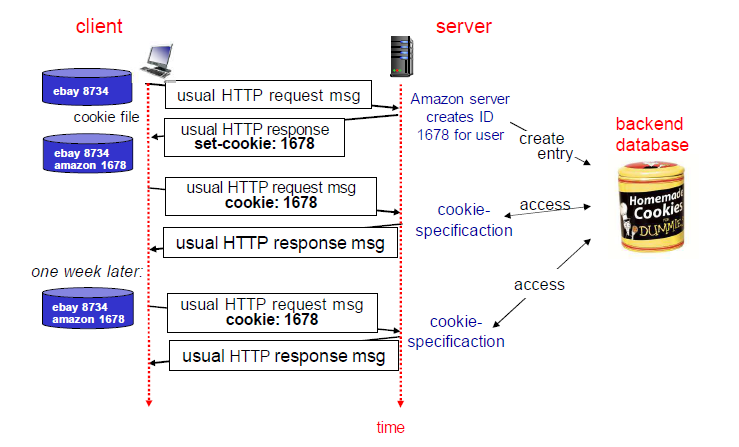
\includegraphics[width=0.75\linewidth]{./images/biscotti.png}
\end{figure}

\subsubsection{I cookies - rappresentano un rischio per la privacy degli utenti?}
Seppur apparentemente convenienti, i cookies sono in tutto e per tutto \textbf{un rischio per la privacy} degli utenti che li accettano. In particolare, se i \textbf{cookie di prima parte} tracciano azioni dell'utente solo sul sito da esso visitato, i tanto sentiti \textbf{cookie di terze parti} permettono di tracciare le azioni degli utenti anche a siti \textbf{non visitati in maniera diretta}, ma semplicemente in quanto embedded in altri siti.

\begin{enumerate}
    \item \verb|GET| da parte del client ad un sito $A$: cookie di terze parti vengono accettati.
    \item Le informazioni prese dal cookie del sito $A$ vengono prelevate anche da siti di terze parti (integrati nella pagina, embedded), e quindi finiscono anche nel database back-end di un sito $B$.
    \item Supponiamo il sito esterno sia embedded in un altro sito $C$. Se lo stesso client è che ha visitato il sito $A$, visiterà anche il sito $C$, il sito $B$ otterrà entrambe le informazioni, potendo effettivamente costruire uno storico dell'attività dell'utente.
\end{enumerate}

Gli utenti e le loro attività online, possono essere tracciate, soprattutto se ai cookies associamo meccanismi di identificazione univoci! Il \textbf{Regolamento Generale sulla Protezione dei Dati} stabilisce e regolamenta l'integrazione dei cookies nei siti web, garantendo che i cookies \textit{analytics} e non essenziali (non-tecnici) possano essere bloccati.

\begin{figure}[htp]
    \centering
    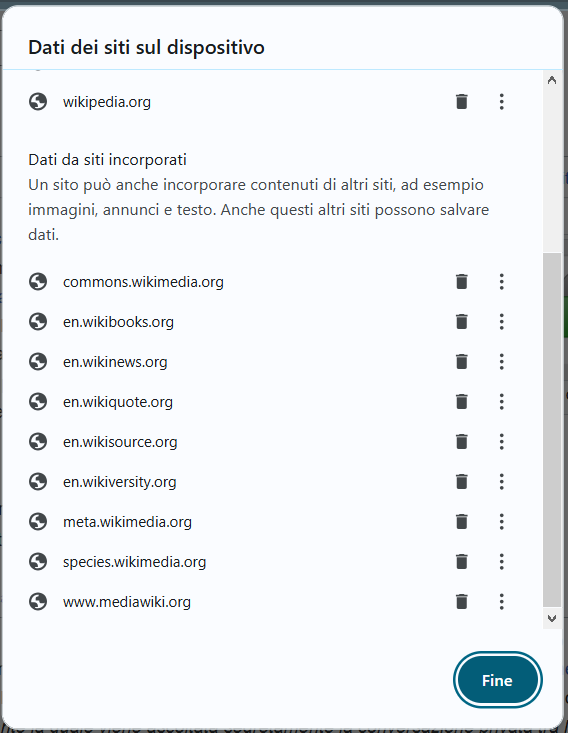
\includegraphics[width=0.5\linewidth]{./images/embeddedcookies.png}
    \caption{Cookies di pagine embedded a wikipedia.org}
\end{figure}
\subsection{DHTML}
È possibile anche costruire una pagina web dinamica col Dynamic HTML: è un insieme di tecnologie che permettono di costruire pagine web con rendering dinamico in funzione dell'utente. Queste tecnologie includono JavaScript e fogli di stile CSS.

\subsubsection{HTTP in breve}
HyperText Transfer Protocol permette agli host di richiedere oggetti (pagine HTML, media e altro) ad un Web Server, e al Web server di rispondere, tramite opportune richieste e risposte HTTP. Usa TCP (sfruttato in maniera differente tra le varie versioni di HTTP), sulla porta 80 del server. Architettura client-server. È stateless, ma possono essere annesse funzionalità stateful tramite l'ausilio di cookies, con i pro e contro del caso. 


\section{Server proxy}
È un server intermedio che permette di \textbf{controllare}, \textbf{filtrare} e \textbf{mascherare il traffico} da parte di uno o più client. Nello specifico:
\begin{enumerate}
    \item I client mandano le richieste al proxy.
    \item Il proxy le invia al server destinazione.
    \item Il server riceve la richiesta del proxy.
    \item Il server invia la risposta al proxy.
    \item Il proxy invia la risposta del server al client originale.
\end{enumerate}

I proxy server si prestano alla perfezione per mascherare IP e monitorare le richieste da parte degli host che li usano.
\newpage

\section{SMTP}
Il \textbf{Simple Mail Transfer Protocol} è un protocollo di invio di e-mail. Si occupa del trasferimento dei messaggi dal mail server del mittente a quello del destinatario.
Usa il protocollo \textbf{TCP} e sulla \textbf{porta 25}.

\begin{itemize}
    \item \textbf{User Agent}.\\
    Software che permette agli utenti di leggere, rispondere, inoltrare, salvare e comporre messaggi. Sono i comuni Microsoft Outlook, Apple Mail, Google Gmail. Permettono di inserire o leggere messaggi sul mail server.
    \item \textbf{Mail Server}.\\
    È il server di posta da cui vengono recuperati, prelevati e inviati i messaggi. Se i due client non sono connessi allo stesso mail server, allora avviene un trasferimento tra i due mail server.
\end{itemize}

\subsection{Le tre fasi di SMTP}
\begin{enumerate}
    \item \textbf{Handshaking.}\\
    Connessione alla \textbf{porta 25} del mail server, il client si identifica tramite il comando \verb|HELO|, il server invia un messaggio di benvenuto.
    
    \item \textbf{Transfer of messages.}\\
    \verb|> MAIL FROM: <indirizzo@email.com>| per specificare email del mittente. \\
    \verb|> RCPT TO: <destinatario@email.it>| per specificare i destinatari. \\
    \verb|> DATA| per iniziare a scrivere la propria mail. Si può andare a capo, una mail si chiude con una riga con esclusivamente il carattere "\verb|.|".
    Si può ripetere questo passaggio per scrivere più mail: queste verranno mandate tutte assieme con la \textbf{stessa sessione TCP} persistente.
    
    \item \textbf{Closure.}\\
    \verb|> QUIT|. Viene chiusa la connessione.
\end{enumerate}


\begin{table}[htp]
    \centering
    \begin{tabular}{|c|p{9cm}|}
        \hline
        \textbf{Header} & \textbf{Significato}\\
        \hline
        \cellcolor{blue!25}To: & Indirizzi e-mail dei destinatari primari\\
        \hline
        Cc: & Indirizzi e-mail dei destinatari secondari\\
        \hline
        Bcc: & Come Cc: ma gli indirizzi e-mail non sono visibili\\
        \hline
        \cellcolor{blue!25}From: & Indirizzo e-mail di chi ha scritto il messaggio\\
        \hline
        Sender: & Indirizzo e-mail dell'effettivo mittente\\
        \hline
        Received: & Ogni server attraverso cui passa la mail lascia
        una traccia in questo campo\\
        \hline
        Return Path: & Può identificare un cammino a ritroso verso il mittente\\
        \hline
        Date: & Data e ora di invio\\
        \hline
        Reply-to: & Indirizzo e-mail a cui le risposte dovrebbero essere inviate\\
        \hline
        Message-id: & Id univoco del messaggio\\
        \hline
        In-Reply-To:& Id del messaggio a cui si è risposto\\
        \hline
        References: & Altri id di messaggi\\
        \hline
        Keywords: & Parole chiave scelte dall'utente\\
        \hline
        \cellcolor{blue!25} Subject: & Breve riepilogo del contenuto del messaggio\\
        \hline
    \end{tabular}
    \caption{Tutti gli header dell'SMTP. In blu, i campi obbligatori}
\end{table}

\subsubsection{Sugli allegati}
Gli \textbf{allegati} delle e-mail sono trasferiti tramite il protocollo \textbf{MIME} (Multipurpose Internet Mail Extension).

\newpage

\subsection{Protocolli del mail server - POP3 e IMAP}
Erroneamente, si potrebbe pensare che il Mail Server giri localmente all'interno della macchina dell'utente. Tuttavia, questo obbligherebbe ogni utente a tenere il proprio dispositivo sempre acceso e in ascolto sulla rete, per assicurare che non venga persa alcuna mail: il server non sarebbe sempre attivo, caratteristica che nel paradigma client-server è fondamentale. Deleghiamo quindi la gestione del \textit{pull} delle e-mail dal Mail Server a dei protocolli, riservando il \textit{push} al protocollo SMTP.

\begin{itemize}
    \item \textbf{IMAP.}\\
    Internet Message Access Protocol. Memorizza le e-mail sul mail server. Questo permette l'accesso alle stesse e-mail da più dispositivi, e grava meno sulla memoria. Usa TCP sulla porta 143 (non crittografata) e 993 (crittografata).
    \item \textbf{POP3.}\\
    Post Office Protocol. Memorizza le e-mail in locale sulla macchina dell'utente, rimuovendole dal Mail Server, non supportando la sincronizzazione delle e-mail su più dispositivi. Usa TCP sulla porta 110 (non crittografata) e 995 (crittografata).
\end{itemize}

\begin{figure}[htp]
    \centering
    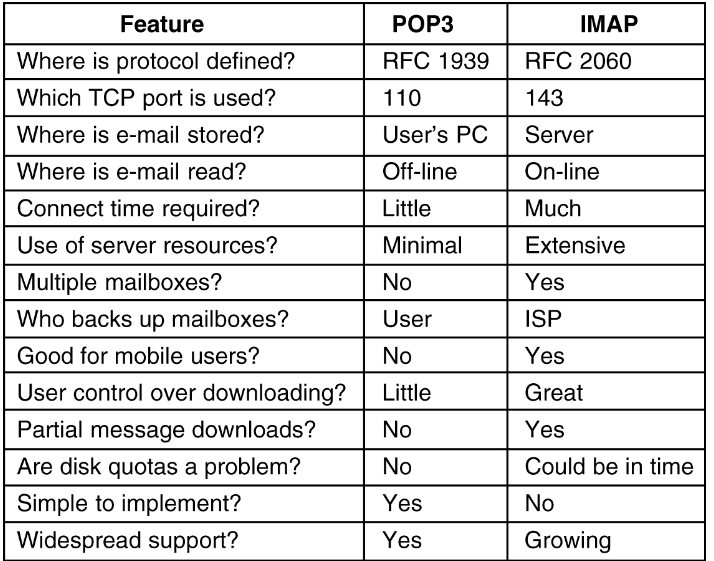
\includegraphics[width=0.75\linewidth]{./images/pop3imap.png}
    \caption{Protocolli POP3 e IMAP a confronto}
\end{figure}

\subsubsection{SMTP, POP3 e IMAP in breve}
\begin{itemize}
    \item \textbf{Simple Mail Transfer Protocol} offre modo al client di mandare, \textit{pushare}, email ad un Mail Server. Usa TCP sulla porta 25 del mail server.
    \item \textbf{Postal Office Protocol} (POP3) permette al client di scaricare, \textit{pullare}, in locale le proprie e-mail, ma solo su un dispositivo. Nel mail server non rimarrà traccia di email che sono state prelevate con questo protocollo. Usa TCP sulla porta 110 del mail server.
    \item \textbf{Internet Message Access Protocol} (IMAP) permette al client di accedere alle e-mail presenti nella propria casella postale del mail server. Non grava sulla memoria del dispositivo, e permette l'accesso da più dispositivi. Usa TCP sulla porta 143 del mail server.
\end{itemize}
\newpage

\section{DNS - Domain Name System}
Gli indirizzi \textbf{IP} \textbf{identificano in maniera univoca gli host in rete} e la loro locazione: la struttura di un indirizzo IP, fornisce infatti informazioni sulla struttura della (sotto)rete e la \textbf{posizione dell'host} all'interno di essa. 
Gli IP \textbf{non sono facili da ricordare}, per un umano, in quanto costituiti esclusivamente da \textbf{caratteri numerici}. Gli \textit{hostname} nascono con lo scopo di associare \textbf{un nome a un IP}: diventa però necessario introdurre un meccanismo che permetta la traduzione degli hostname in indirizzi IP. Nasce così il DNS.
\begin{verbatim}
        151.97.240.12   <-   www.dmi.unict.it
        151.97.240.4    <-   www.unict.it
        151.97.6.236    <-   www.ing.unict.it
        151.97.252.132  <-   galileo.dmi.unict.it
\end{verbatim}

Il protocollo DNS supporta inoltre:
\begin{itemize}
    \item \textbf{Alias names} sugli hostname canonici. 
    \item Gestione dei reindirizzamenti nel caso di cambio di indirizzo IP del sito.
    \item Distribuzione del carico su più server (tra server DNS primari e secondari).
\end{itemize}

\subsection{DNS - Transport Layer}
Le richieste \textbf{sono mandate} alla \textbf{porta 53} dei server DNS. Il protocollo usa \textbf{sia UDP}, che \textbf{TCP}. Per le banali query del servizio, si predilige UDP, e TCP è riservato per risolvere circostanze particolari, come informazioni troncate.
TCP è sempre usato durante gli \textbf{zone transfer}, ossia quando un DNS primario vuole effettuare una copia dei suoi record ad uno o più server DNS secondari.

\subsection{Struttura del DNS}
È un \textbf{database distribuito}, con una \textbf{struttura gerarchica} ad albero che \textbf{velocizza la ricerca dell'IP}.\\
Individuiamo le classi di DNS della gerarchia:

\begin{itemize}
    \item \textbf{Root server.}\\
    Contengono gli indirizzi IP del TLD server. I root server sono 13, gestiti da 12 aziende, e nel complesso si hanno più di 1000 copie di questi record.
    \item \textbf{Top-Level Domain Server.}\\
    Si occupano degli indirizzi IP dei server autoritativi, e sono organizzati per domini di primo (\verb|.com .gov .org .net .edu|) e di secondo livello (\verb|.it .uk .us|).

    \item \textbf{Authoritative Domain Name Server.}\\
    Effettuano l'ultima associazione indirizzo IP - hostname.
\end{itemize}

Su questa struttura gerarchica, aggiungiamo anche una \textbf{distribuzione del carico di lavoro} tra più server (\textbf{primari} e \textbf{secondari}), \textbf{meccanismi di caching} vari e \textbf{distribuzione di questi server a scala mondiale}: questi fattori rendono il DNS uno dei servizi più \textbf{robusti} (gestione non centralizzata), \textbf{affidabili} e \textbf{veloci} della rete.

\begin{figure}[htp]
    \centering
    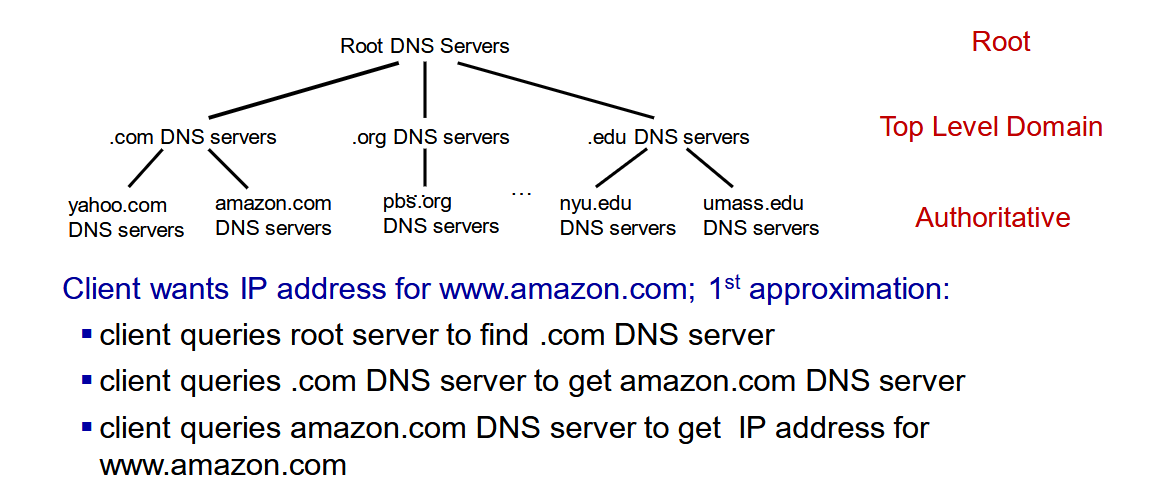
\includegraphics[width=0.75\linewidth]{./images/gerarchiadns.png}
\end{figure}

\subsection{Primary e secondary DNS}
A causa dell'\textbf{alto numero di richieste} ai server DNS, \textbf{a ogni DNS primario}, contenente le copie originali dei record in modalità lettura e scrittura, \textbf{coincidono molteplici DNS secondari}, contenenti \textbf{copie di sola lettura}. Lo scopo è quello di \textbf{bilanciare il carico} di lavoro tra i DNS.



\subsection{Name resolution - Modo iterativo}
\begin{figure}[htp]
    \centering
    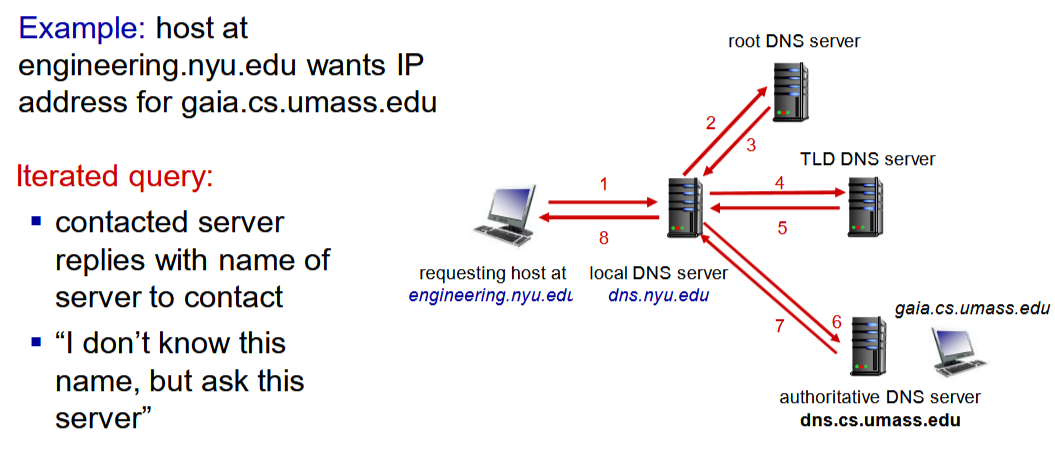
\includegraphics[width=0.75\linewidth]{./images/iterative.png}
\end{figure}

Le query iterative offrono una strategia di controllo che \textbf{distribuisce bene il carico} sui vari server. Tuttavia, il client dovrà gestire molte più richieste, una per DNS coinvolto. (N.B. la prima query dell'immagine è ricorsiva!)

\subsection{Name resolution - Modo ricorsivo}
\begin{figure}[htp]
    \centering
    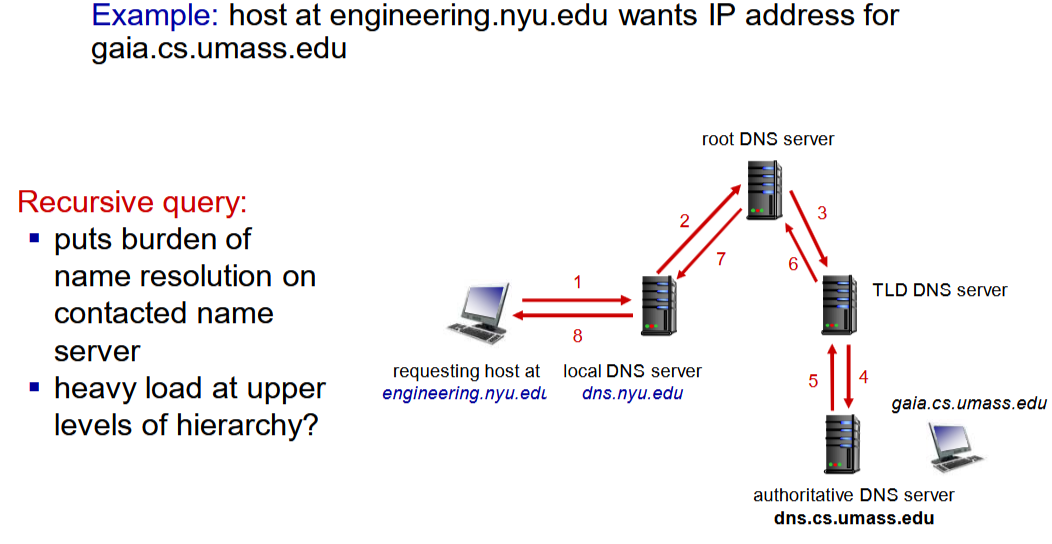
\includegraphics[width=0.75\linewidth]{./images/recur.png}
\end{figure}

Le query ricorsive offrono una \textbf{risposta diretta} al client \textbf{senza ulteriori richieste} da mandare. Ogni server comunicherà con quello successivo e quello precedente (\textbf{favorendo il caching}, i server DNS si scambieranno le loro risposte), con una logica molto più semplice di quella iterativa. Tuttavia, a causa della ricorsione, si avrà \textbf{maggiore latenza} (soprattutto quando non avvengono cache hit), e \textbf{maggior carico di lavoro} sulla parte alta della gerarchia dei server DNS. 

\subsection{Caching e Updating DNS}
Ogni volta che un qualunque DNS Server (name server) riceve una risposta e “impara” come mappare una determinata informazione, la \textbf{memorizza nella propria cache} per evitare future richieste nella gerarchia di risoluzione. Ciò permette di ridurre il carico sui server e migliorare le prestazioni. Tipicamente, i TLD server vengono memorizzati nella cache dei DNS locali per ridurre le query ai root. Le entry delle cache (anche quelle locali) devono essere \textbf{aggiornate periodicamente} dopo un tempo identificato dal \textbf{TTL} (Time To Live): esso è un valore associato ai record DNS che indica per quanto tempo un resolver DNS \textbf{può mantenere nella cache una risposta prima di doverla aggiornare}. Il caching velocizza significativamente il funzionamento dei DNS. Un cache hit eviterà la richieste a tutti DNS server dei livelli inferiori della gerarchia: per questo la cache di ciascun DNS è il \textbf{primo elemento che viene consultato per qualsiasi richiesta}. Una cache hit è sempre un grande vantaggio in termini di velocità.

\newpage

\subsection{Forma di un record di un DNS}
\begin{verbatim}
RR format: (name, value, type, ttl)
\end{verbatim}
\begin{itemize}
    \item type=A:\\
    \verb|name| è l'hostname, \verb|value| è l'IP address
    
    \item type=NS:\\
    \verb|name| è il dominio, \verb|value| è l'hostname del server autoritativo su questo dominio.
    
    \item type=CNAME\\
    Canonical Name. \verb|name| è un alias per il nome canonico \verb|value|.

    \item type=MX\\
    \verb|value| è il nome del mail server associato all'hostname \verb|name|.
\end{itemize}

\subsection{Forma di un messaggio DNS}
Formato uguale tra query e risposte.
\begin{figure}[htp]
    \centering
    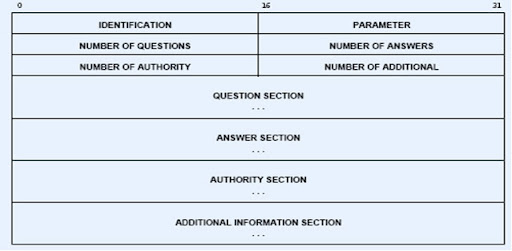
\includegraphics[width=1\linewidth]{./images/dnsmex.png}
\end{figure}

\begin{itemize}
    \item \textbf{Sezione di intestazione.}\\
    Sono i primi 12 byte, e contiene vari campi.
    \begin{itemize}
        \item Identificazione, 16 bit. Permette di associare risposte a richieste.
        \item Flag, 16 bit. Tra questi, un bit che specifica \verb|query/reply|.
        \item Numero di domande, numero record di risposta, numero record autoritativi, numero record addizionali.
        Specificano il numero di record e domande delle prossime sezioni. Ognuno è un numero a 16 bit.
    \end{itemize}

    \item \textbf{Sezione delle domande.}\\
    Include informazioni relative alle richieste che stanno per essere effettuate, un campo con il nome richiesto e uno con il tipo di domanda sul nome richiesto.

    \item \textbf{Sezione delle risposte.}\\
    Presente nei messaggi di risposta. I record contengono al loro interno le informazioni specificate nel paragrafo precedente. Una risposta può tornare più indirizzi.

    \item \textbf{Sezione autoritativa.}\\
    Contiene record di altri server autoritativi.

    \item \textbf{Sezione aggiuntiva.}\\
    Contiene altri record utili correlati alla richiesta.
\end{itemize}

\newpage

\subsection{nslookup}
Questo programma permette di effettuare richieste DNS a un determinato dominio.
\begin{verbatim}
> nslookup
Server predefinito:  vodafone.station
Address:  **indirizzo mac**

> wikipedia.com
Server:  vodafone.station
Address:  **indirizzo mac**

Risposta da un server non autorevole:
Nome:    wikipedia.com
Addresses:  2a02:ec80:600:ed1a::3           //IPv6
          185.15.58.226                     //IPv4

> overleaf.com
Server:  vodafone.station
Address:  **indirizzo mac**

Risposta da un server non autorevole:
Nome:    overleaf.com
Address:  34.120.52.64                  

> overleaf.it
Server:  vodafone.station
Address:  **indirizzo mac**

*** vodafone.station non è in grado di trovare overleaf.it: Non-existent domain
\end{verbatim}

\subsection{Problemi di sicurezza e criticità dei DNS}
\begin{itemize}
    \item \textbf{DDoS attacks su Root Server}.\\
    Consiste nel sovraccaricamento di un DNS root tramite richieste spazzatura. Il traffic filtering può essere una soluzione per filtrare il traffico osservando la semantica degli URL. Questo approccio potrebbe rifiutare richieste da utenti reali. Al giorno d'oggi, a questo scopo, vengono sfruttate alcune tecniche d'intelligenza artificiale.
    Un'altra soluzione può essere mantenere una lista di IP di TLD server notoriamente non malevoli.
    
    \item \textbf{Man-in-the-middle}.\\
    Un attacco che consiste nell'intercettare le richieste tra i DNS.
    
    \item \textbf{DNS poisoning/DNS spoofing}.\\
    Consiste nel sostituire risposte DNS effettive con risposte fittizie, ottenendo un \textbf{reindirizzamento errato}. I danni da DNS poisoning si propagano \textbf{a lungo termine}, a causa del \textbf{caching}.
\end{itemize}

\subsubsection{DNS in breve}
Risoluzione degli hostname in indirizzi IP. UDP (ma anche TCP), porta 53 del server ricevente. Architettura client-server. Sfrutta un sistema di server distribuiti, e organizzati in maniera gerarchica, per facilitare la ricerca. Meccanismi di caching, distribuzione del carico su server primari e secondari, e in generale l'alto numero di server nel mondo, offrondo un sistema solido e veloce.

\newpage

\section{SNMP}
Il \textbf{Simple Network Management Protocol} è un protocollo di rete \textbf{connectionless} che permette la \textbf{gestione di una rete} e il \textbf{monitoraggio dei dispositivi} ad essa collegati. Gli \textbf{amministratori} possono raccogliere informazioni sulle prestazioni e lo stato dei dispositivi.

\subsection{Attori del SNMP}
\begin{itemize}
    \item \textbf{Manager SNMP.}\\
    Applicazione che comunica con i dispositivi della rete, per raccogliere informazioni. Può inviare richieste agli agenti SNMP.
    
    \item \textbf{Agente SNMP.}\\
    È un software presente in ogni dispositivo della rete da monitorare. Raccoglie informazioni relativi al dispositivo (quali stato, configurazione, prestazioni, etc.) e risponde alle richieste del manager con queste informazioni.
    
    \item \textbf{MIB (Management Information Base).}\\
    È un database, presente in ogni agente SNMP, che definisce le informazioni che possono essere raccolte o modificare tramite SNMP.
    
    \item \textbf{Protocollo SNMP.}\\
    È il protocollo vero e proprio utilizzato nella comunicazione tra agenti e manager. È basato sul paradigma client-server. Il manager è il client, l'agente fa da server.
\end{itemize}
Usa il protocollo \textbf{UDP} e la\textbf{porta 161} degli agenti per mandare messaggi, e la \textbf{porta 162} del manager per ricevere le \textbf{notifiche} (\textit{traps}).\\
Le \textbf{traps} sono generate successivamente a \textbf{malfunzionamenti, eventi e anomalie}.

\subsection{Messaggi SNMP}
\subsubsection{Da manager a agente}
\begin{itemize}
    \item \verb|GetRequest|.\\
    Richiesta di recupero del valore di una variabile.
    \item \verb|SetRequest|.\\
    Richiesta di cambiamento del valore di una variabile.
    \item \verb|GetNextRequest|.\\
    Richiesta di recupero di possibili variabili e dei loro valori.
\end{itemize}

\subsubsection{Da agente a manager}
\begin{itemize}
    \item \verb|GetResponse|.\\
    Restituisce il valore di una o più variabili.
    \item \verb|Trap|.\\
    Notifica in maniera asincrona e senza richiesta del manager situazioni anomale o eventi significativi della rete.
\end{itemize}

\subsection{Versioni di SNMP}
La prima versione di SNMP presentava numerose criticità in termini di sicurezza e performance migliorabili. La seconda e la terza versione migliorano la sicurezza del protocollo, le performance. In particolare con la terza versione, viene introdotta la crittografia per i dati e un sistema di autenticazione.

\subsubsection{SNMP in breve}
\textbf{Simple Network Management Protocol} offre un servizio per la gestione. UDP, \textbf{porta 161 degli agenti}, \textbf{porta 162 del manager}. Architettura client-server: i server sono gli agenti. Ogni dispositivo agente ha una base di dati contenente oggetti per gestire i dispositivi di rete e i loro attributi. I dispositivi possono segnalare anomalie al manager tramite delle traps. È un protocollo \textbf{connectionless} con \textbf{comunicazioni asincrone}.

